\label{chap4}
\section{Basic assumptions}

The aim of this work is to propose a \gls{knx} prototype, applicable for environments with increased availability demands.
The prototype should be designed in a transparent way, utilizing a "plug and play" functionality to build a secure \gls{knx} network.
This means that a device outside of this network, unaware of
the secured \gls{knx} network, should be able to deliver through and receive messages from such a secured network without any prerequisites. 
Every device with one connection to an unsecured \gls{knx} network (called cleartext \gls{knx} line) and two distinct connections to a secured \gls{knx}
network (called secure lines), running the master daemon, will work
as a security gateway. Thus, the presence of at least two of these security gateways connected to each other by two secure lines will constitute a 
secured \gls{knx} area, bridging between areas with increased security demands, as shown in Figure \ref{fig:secArea}.
\\
\\
The basic tasks of such a security gateway consist of:
\begin{itemize}
 \item establishing keys with its communication partners within the secured \gls{knx} network (the security gateways)
% \item maintaining some kind of synchronization token between all security gateways
 \item providing redundant communication lines, achieving improved availability by encrypting and authenticating all messages which are received on the unsecured line, and delivering them to the proper security gateways which act as
 border device for the given group address, using both secure lines
 \item checking all messages which are received on the secured lines for integrity and authenticity, removing duplicates, unwrapping and delivering them to
 the unsecured area
\end{itemize}

\subsection{Security related architectural overview}

As stated in Section \ref{sec:knxTransportLayer}, different possibilities for communication within a \gls{knx} network are possible: point to point, multicast and broadcast.
To introduce as little additional traffic into the network as possible, a sound concept for translating clear- to secure-\gls{knx} addresses (and vice versa) has to
be defined. While in principle it would be possible to use the communication modes in a transparent way (i.e., point-to-point in unsecured \gls{knx} translates
to point-to-point in secured \gls{knx}, and vice versa, and so on), this approach leads to some serious problems, rendering this solution impracticable:
due to the topology of \gls{knx}, it is impossible to know a priori the exact physical location of a device (i.e., its \gls{ia}). Additionally,
every device can be member of an arbitrary number of group addresses (bounded by the maximum number of group addresses), which also is not known in advance.
Group-membership may also be subject to change and therefore complicates the situation. Finally, devices can leave or join the network at every moment by powering the
device up or down.
\\
Therefore, a device which receives a message on its unsecured \gls{knx} line, examining the destination address, simply does
not know which device(s), if any, will be the gateway(s) responsible for delivering this datagram one hop toward its final destination,
regardless if the destination address is a \gls{ia} or a \gls{ga}.
\begin{figure}
    \centering
    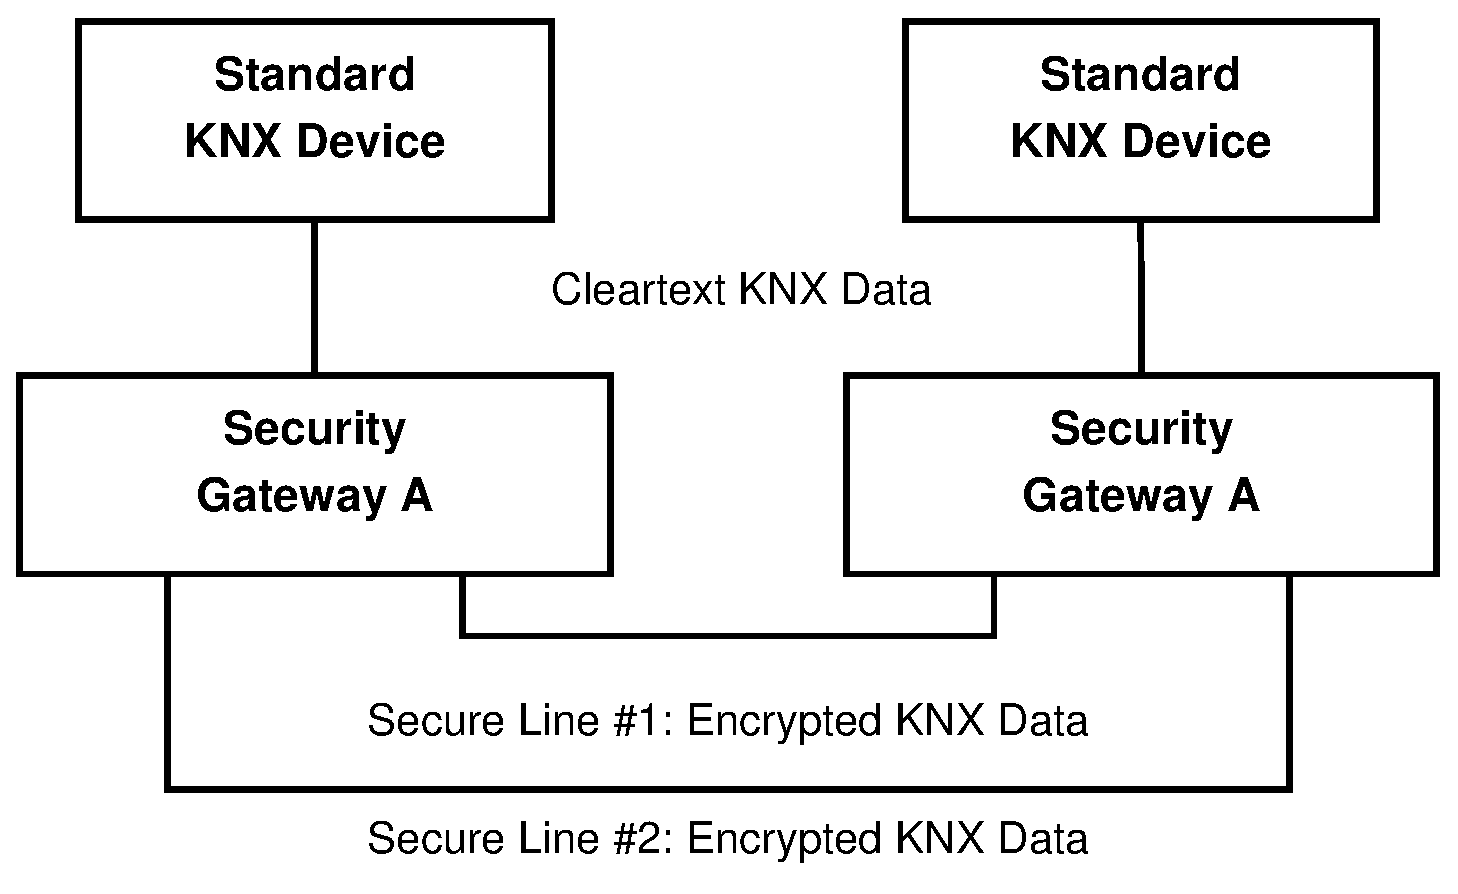
\includegraphics[width=0.8\textwidth]{figures/SecureArea.eps}
    \caption{Secure Area}
    \label{fig:secArea}
\end{figure}
\\
\\
A straightforward solution to this problem would be to wrap every datagram which enters the secured \gls{knx} network via a security gateway into a new, properly secured
broadcast datagram, and delivering this new package to the secured \gls{knx} network. Then, the package would be available to all other security gateways, which
will unwrap it and forward the resulting inner datagram to its unsecured \gls{knx} line. If the destination address (group or individual) of the actual payload
is assigned to a device connected
to the unsecured \gls{knx} network, the device holding this \gls{ia} or \gls{ga} will recognize it and the package will reach its destination. 
Otherwise it will simply be discarded.
\\
A serious constraint rising from this broadcast approach is that a single,
global network key must be used, because every security gateway must be able to decrypt and check every package which it receives on its secured lines,
even if it does not serve as gateway to the wanted group address. 
The key of course can be renegotiated among the security gateways at every time, but this approach is considered
unsecure because an attacker can target \textit{any} of the security gateways constituting the secure network. An adversary breaking one single device gains
access to the network traffic of all devices. This could be achieved by physical access to any of the security gateways, for example by reading out the
memory of the device, and thus obtaining the globally used network key. This way, the network traffic can be decrypted by the adversary as long as no new
key is renegotiated. Another problem is that multi-party key negotiation is a costly task if a public-private key scheme
is to be used: as shown in Figures \ref{fig:dh1} and \ref{fig:dh2}, a lot of messages have to be exchanged before an encryption can be done. 
\\
\\
To encounter these problems, different keys must be used, thus achieving pairwise end-to-end encryption between all devices. 
%This way it is also possible to achieve different security levels, depending on the function a 
%particular unsecured \gls{knx} device fulfills. It would be possible, for example, to distinguish between 'normal' gateways and 'hardened'
%gateways which are specially guarded against physical access, for example by applying physical intrusion detection. Thus,
%the risk of breaking the whole system is reduced, because breaking a device in one security level does not affect the security of the devices with other
%security levels.
%So, for breaking all $n$ security levels of a system, at least $n$ devices, all belonging to different levels must be broken.
%As a motivating example, imagine a setup which consists of window controls in an upper floor, and door controls in the
%base level. Obviously, the security constraints for the latter one would be higher. By using normal devices for window control, and hardened devices for
%door control, a security firewall can be deployed, thus containing the damage an adversary can do to the whole system.
Figure \ref{fig:firewall} shows the logical connections within a \gls{knx} network using end-to-end encryption. An 
attack of node $A$ can only compromise keys known to the device, thus effectively separating communication between the nodes $B$, $C$, and $D$ from
the attacker.
% \begin{figure}
% \centering
% \begin{tikzpicture}[scale=0.2]
% \tikzstyle{every node}+=[inner sep=2pt]
% \tikzstyle{arrow}=[draw, -latex] 
% \tikzset{
%     pil/.style={
%            ->,
%            thick,
%            shorten <=1pt,
%            shorten >=1pt,}
% }
% 
% \usetikzlibrary{automata,positioning}
% \usetikzlibrary{positioning}
% 
% \node[state,text width=1.5cm,align=center]					at (-20,0)		(a)		{A}; 
% \node[state,text width=1.5cm,align=center]					at (5,0)			(b)		{B}; 
% \node[state,text width=1.5cm,align=center]					at (30,15)		(c)		{C}; 
% \node[state,text width=1.5cm,align=center]					at (30,-15)	(d)		{D}; 
% 
% \path[pil,<->] (a)  edge[]   node[text width=1cm] {$KEY_{AB}$} (b);
% \path[pil,<->] (b)  edge[]   node[text width=3cm,align=left] {$KEY_{BD}$} (d); 
% \path[pil,<->] (b)  edge[]   node[text width=3cm,align=left] {$KEY_{BC}$} (c); 
% \path[pil,<->] (d)  edge[]   node[text width=3.5cm,align=right] {$KEY_{CD}$} (c); 
% \end{tikzpicture}
% \end{figure}
\\
\\
\begin{figure}
  \centering
   % 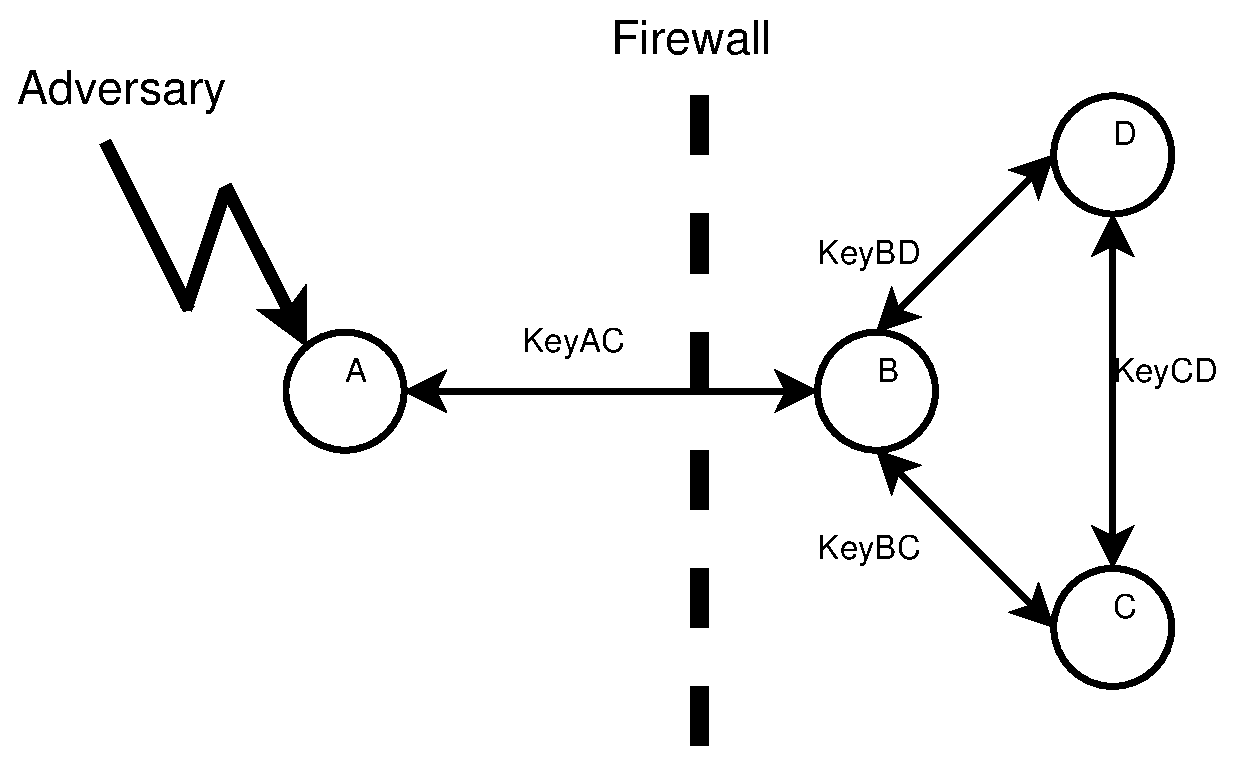
\includegraphics[width=0.8\textwidth]{figures/firewall.eps}
   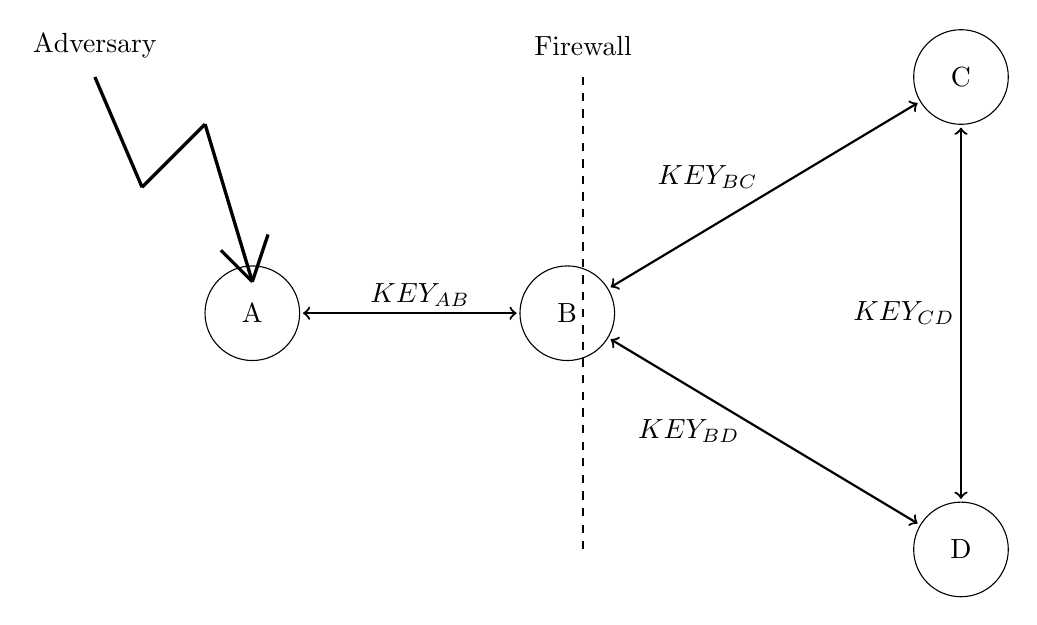
\begin{tikzpicture}[scale=0.2]
\tikzstyle{every node}+=[inner sep=2pt]
\tikzstyle{arrow}=[draw, -latex] 
\tikzset{
    pil/.style={
           ->,
           thick,
           shorten <=1pt,
           shorten >=1pt,}
}

\usetikzlibrary{automata,positioning}
\usetikzlibrary{positioning}

\node[state,text width=1.0cm,align=center]					at (-15,0)		(a)		{A}; 
\node[state,text width=1.0cm,align=center]					at (5,0)			(b)		{B}; 
\node[state,text width=1.0cm,align=center]					at (30,15)		(c)		{C}; 
\node[state,text width=1.0cm,align=center]					at (30,-15)	(d)		{D}; 

\path[pil,<->] (a)  edge[auto]   node[text width=1cm] {$KEY_{AB}$} (b);
\path[pil,<->] (b)  edge[]   node[text width=3.2cm,align=left] {$KEY_{BD}$} (d); 
\path[pil,<->] (b)  edge[auto]   node[align=left] {$KEY_{BC}$} (c); 
\path[pil,<->] (d)  edge[auto]   node[] {$KEY_{CD}$} (c); 

\draw [dashed] (6,-15) -- (6,15);
\node[] at (6,17) {Firewall};
\draw [very thick] (-25,15) -- (-22,8);
\draw [very thick] (-22,8) -- (-18,12);
\draw [very thick] (-18,12) -- (-15,2);
\draw [very thick] (-14,5) -- (-15,2);
\draw [very thick] (-17,4) -- (-15,2);
\node[] at (-25,17) {Adversary};

\end{tikzpicture}
 \caption{Firewall}
 \label{fig:firewall}
\end{figure}
As stated above, to be able to use different keys every security gateway has to know how to reach a given address so that the data can be encrypted
exclusively for the responsible gateway. The solution to this problem is to maintain some kind of routing table, mapping \glspl{ga} and \glspl{ia} of unsecured
\gls{knx} devices to \glspl{ia} of responsible security gateways.
Such a routing table can be built statically at setup time, with the obvious disadvantage
that the exact topology of the applied network has to be known in advance, thus reducing the flexibility. Here, every security gateway holds a static 
table which consists of mappings between \glspl{ia} or \glspl{ga} of unsecured \gls{knx} devices and \glspl{ia} of security gateways at the border
between the secured and the unsecured \gls{knx} network, as well as all keys used for the particular security level the gateway belongs to.
This table would be generated once, after the topology of the network has been fixed, and must be equipped with the proper keys and can then
be copied to the security gateways constituting the secured \gls{knx} area. New security gateways can be deployed as long as they only introduce sending 
unsecured \gls{knx} devices, whose recipients are already known group addresses behind existing security gateways. A new group address, introduced by a newly installed device behind
an already existing security gateway, will not be reachable, simply because the routing information is not available. 
Another disadvantage is that the deployment of new
security gateways, connecting devices with new or already known \glspl{ga}, is impossible as the \gls{ia} of the new gateway - which of
course must be unique - is unknown to the existing setup, thus making the new unsecured \gls{knx} devices unreachable.
\\
To tackle this problem, another approach would be to build this mapping table dynamically. Therefore, every security gateway must periodically poll
on its unsecured lines for \gls{knx} devices, thus populating a list of reachable \gls{knx} devices. Whenever a 
device wants to send data to a group address, it has to process a lookup first to obtain the \glspl{ia} of the responsible security gateways: the lookup
must contain the wanted group address, as well as the sender's public key.
Every 
gateway which finds the wanted group address in its group list must reply with an according message to the requester, thus announcing that it is responsible
for delivering data to the wanted group address, and must also publish its own public key, thus allowing pairwise end-to-end encryption.
This procedure requires no a priori knowledge of
the network topology, so security gateways can be added to the network as well as unsecured \gls{knx} devices behind new or existing gateways at any time. This
flexibility of course has to be purchased with increased complexity as well as additional traffic introduced into the network.
\\
\\
A middle course is chosen: the reachable group address list is generated whenever a new security gateway is added to the network,
 handling discovery of these \glspl{ga} as described
above. This allows to deploy new security gateways with connected unsecured devices, thus achieving a compromise between flexibility and complexity. 
\\
Sending data to a group address therefore follows the triad discovery request, discovery response and data transfer, shown in Figure \ref{fig:prot1}. Broadcast
messages are depicted as solid end of the arrow, the rest denoting unicast messages.
\begin{figure}
  \centering
    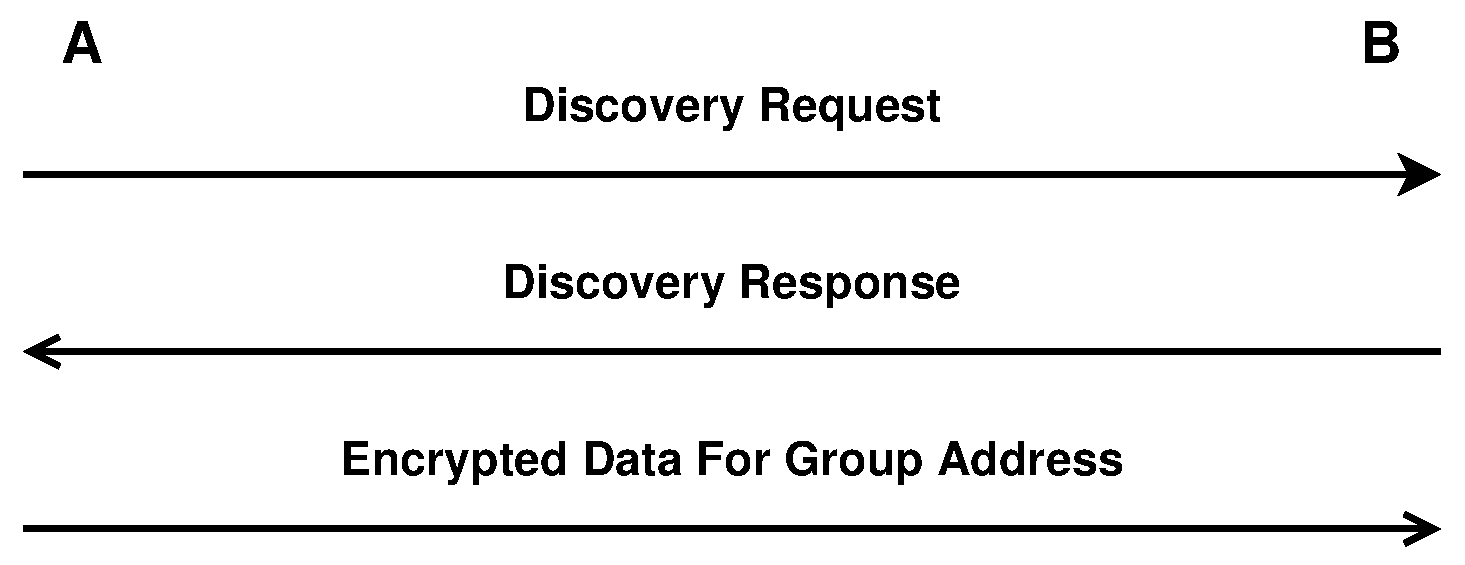
\includegraphics[width=0.95\textwidth]{figures/protokoll1.eps}
 \caption{Communication schema}
 \label{fig:prot1}
\end{figure}
To enable multiple devices to announce responsibility for a group address, the device wanting to transmit data to this group address must accept discovery responses
following its request message for a short time window.
\\
\\
The discovery messages generated by security gateways should be encrypted, too. Although these datagrams don't contain \gls{knx} data per se, they allow
a listening adversary to learn the topology of the network, knowledge which can be valuable for developing an attack strategy, as well as generating meta data.
For example, if an attacker learns that a particular security gateway is responsible for only one group address and further gets knowledge that this 
group address is responsible for switching a light (i.e., by visual observation), the attacker afterwards may be able to derive a personal profile just by detecting
packages for this group address, although the payload of the datagrams to the responsible security gateway are encrypted.
If the discovery messages are encrypted too the adversary doesn't know how many and what
group addresses are behind a specific gateway, and it will be harder to derive personal profiles or to gather knowledge of the network topology.
\\
Discovery request messages must be broadcast messages, readable by all security gateways. To limit the protocol overhead, a global network key is used here.
\\
\\
To provide authenticity, all datagrams passing the secure \gls{knx} network must contain a \gls{mac2} to prevent modification of them.
\\
Defense against replay attacks is achieved by counters. These must be strictly monotonically
increasing and must not overflow. The counters can be compared to an initialization vector that prevents the mapping of same cleartext messages to same ciphertext messages
under the same encryption key.
\\
Two different types of counters are used: one global counter $Ctr_{global}$, used for avoiding replay attacks against discovery messages. A second kind of counter
is used for the actual data transfer. Beside avoiding replay attacks, this counter is necessary to detect and delete duplicates, caused by the redundant network. 
%see \ref{ctrAvail} for details.
\\
Usage of the global counter $Ctr_{global}$ raises another question, namely how a new device gets knowledge of the actual value of $Ctr_{global}$.
Therefore, a synchronization service must be defined, allowing a newly powered up device that wants to join the network to synchronize with the rest of the network, as shown in Figure \ref{fig:syncProt}.
\begin{figure}
  \centering
    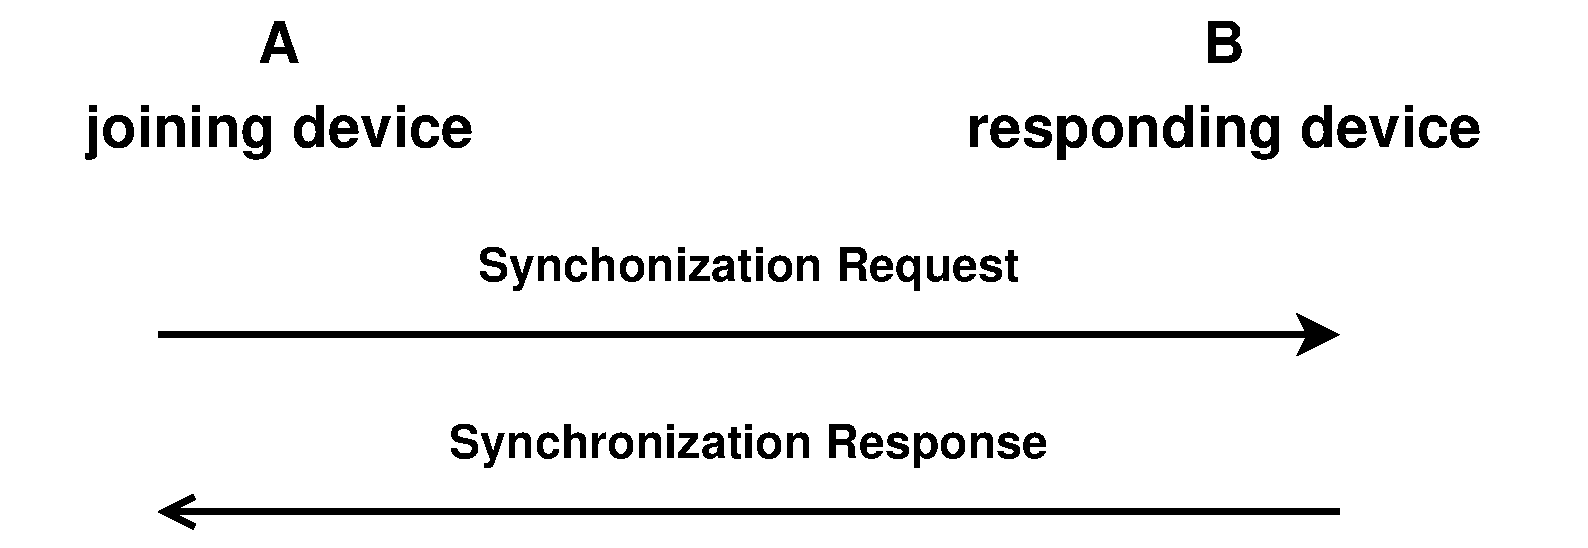
\includegraphics[width=0.8\textwidth]{figures/protSync.eps}
 \caption{Synchronization service}
 \label{fig:syncProt}
\end{figure}
Replay attacks are mitigated by including the current time into \gls{mac2} calculation. Low temporal resolution relaxes time-synchronization issues between
different devices.

\subsubsection{Key management}

While it would be possible to use a centralized concept, no trusted on-line party is used in this work. A centralized approach would need fall-back key servers
which inherit the task of generating and distributing keys and parameters in case of a master key server failure. Otherwise, the network would suffer from a
single point of failure in case no such fall-back mechanism is applied, an assumption that would clearly disqualify the design as highly available.
\\
The following key management is proposed:

\begin{itemize}
 \item A long-term key known to all security gateways is defined. As already stated, this key must be copied to every device at setup time. 
This pre-shared key $k_{psk}$ is used for symmetric encryption and serves different purposes: first, it authenticates synchronization messages.
Secondly, this key $k_{psk}$ is used to encrypt discovery requests and discovery responses.
 %\item $k_{global}$ is used to authenticate and encrypt locally generated and decrypt received discovery requests, as well as to authenticate and encrypt
 %locally generated discovery responses and decrypt received ones. These discovery service datagrams securely transport the third type of keys:
 \item Asymmetric keys are used for end-to-end encryption of the actual data packages between 2 security gateways. \gls{ecdh} serves as key negotiation algorithm.
 To protect against man-in-the-middle attacks, authenticity of the \gls{dh} parameters must be assured.
 \item This is the task of the third kind of keys: another pre-shared key is used to authenticate the \gls{dh} parameters.
\end{itemize}


\subsection{Redundancy related architectural overview}\label{ctrAvail}
 
Whenever a \gls{knx} packet is
generated by a device on an unsecured line (called client), the connected security gateway will read, duplicate and encapsulate it into another \gls{knx} frame 
and then send it over both lines. If both lines are available, i.e., there is, for example, no shortcut, the security gateway responsible for forwarding the frame
will receive two different \gls{knx} frames encapsulating the same
payload, which itself is the \gls{knx} frame generated by the \gls{knx} client device in the first place. 
One message must be discarded to avoid duplicates. 
This is achieved with a monotonically increasing counter that also guards against replay attacks. Whenever a package, generated by a client, enters the
network, a counter for outgoing packages is incremented, called $Ctr_{out}$, and is sent along the message. 
This counter must be unambiguously referenced by the origin cleartext message. 
The receiving side must maintain a counter for incoming packets, called $Ctr_{in}$, which will be updated by the received counter value
as soon as the first frame is received if the received value is higher than the saved one.
Subsequent delivery of the duplicate can be detected because the containing counter value equals the saved counter value.
\\
\\
To identify duplicate frames, basically various possibilities exist:
\\
Referencing both $Ctr_{out}$ and $Ctr_{in}$ by the \gls{ga} of the origin cleartext message does only work if for every destination
 \gls{ga} in the network, at most one sending client device exists. Assuming client device $A$ and afterwards client device $B$ want to send the first message to
 the same destination \gls{ga}, the delivery of the message
 originating from device $A$ will trigger an update of the corresponding counter $Ctr_{in}$ at the responsible gateway, but device $B$ will use its own counter
 for the outgoing message. Because device's $B$ outgoing counter is less than the gateway's actual incoming counter, both frames will be discarded by the gateway.
Therefore, this is no viable solution.
\\
\\
It shows that the easiest way to unambiguously identify duplicates is by referencing both $Ctr_{out}$ and $Ctr_{in}$ by the \gls{ia} of the origin
cleartext message. This solution works despite potential network failures on one or both secure lines, provided that each client device is identified by a unique
\gls{ia}. This is argued as follows:
\\
For simplicity, assume that three security gateways $A$, $B$ and $C$ are connected to each other by two distinct, secured \gls{knx} lines, and each gateway is connected
to an arbitrary number of client devices through their cleartext lines, each with a unique \gls{ia}.
Additionally, each client device is destination for an arbitrary number of \glspl{ga}.
If a security gateway receives a cleartext message, it will at first check the counter value $Ctr_{out}$ for the \gls{ia} and increment it. After that, the 
discovery phase takes place. This discovery request can be answered by zero, one or two other security gateways. If at least one reply is received, the package
is duplicated, encrypted, fitted into a unicast data frame together with $Ctr_{out}$ and sent on both lines.
\\
Every gateway answering the discovery request will be sent 2 duplicate messages, one on each secure line. Now, there are three possibilities:
\begin{itemize}
 \item If both secure lines are available, one data frame will be handled first and the contained counter will be saved as actual $Ctr_{in}$ for the \gls{ia}
 of the inner frame. When handling the second frame, the contained counter will be equal the saved counter, and thus the frame can be discarded.
 \item If only one secure line is available, no duplicate will arrive, but the receiving gateway(s) will nevertheless update the received counter value for the
 \gls{ia}.
 \item If both lines are unavailable, the responsible gateways cannot update the corresponding value for $Ctr_{in}$. Nevertheless, the sending side will 
 increment and update
 the outgoing counter $Ctr_{out}$. As soon as the responsible gateways are reachable again, new data frames will bear an even higher counter than saved on the
 receiving side, thus allowing data transfer to the \gls{ga} again.
\end{itemize}


%If both lines are available, one message will be handled first and trigger an
%incrementation of the corresponding source address counter (i.e., the \gls{ga}).
%The duplicated message, which is handled after that, can safely be discarded because the corresponding counter value will be less than the saved value.

% Nevertheless which package from which secure line is forwarded to the unsecured line, each line must acknowledge
% every received package: this is done by generating a special acknowledge frame which is sent back to the sending gateway. The payload of this package must
% allow the sending gateway to unambiguously identify the acknowledged package, i.e., it must bear source and destination address of the package generated
% by the client, as well as the used counter value. As a consequence, these acknowledgement frames must be encrypted and authenticated as well.
% If no acknowledgement frame is received within time $t_{ACK}$, a retransmission is done on both lines. This retransmission simply re-submits the same
% package with the same counter value again. Regarding the security this is no problem because a passive attacker can not learn anything from such a repeated
% package.


\subsection{Operational constraints}\label{sec:opContraints}

The introduction of encapsulating security gateways implicates that some timing constraints, defined by \gls{knx}, cannot be met:

\begin{itemize}
 \item Acknowledgement frames, used in point-to-point communication, as defined in \gls{knx} and introduced in Section \ref{sec:ackFrame}, cannot be guaranteed to be
 delivered within the specified deadlines: whenever
 a new \gls{knx} datagram is generated by a client, at first the discovery phase has to occur. Only after that the to-acknowledged frame is sent. So there are
 multiple delays introduced, stalling the delivery: the first delay is caused by sending of the discovery package.
 After that, a second delay occurs because the security gateway must wait for the discovery response(s), possibly retransmitting the discovery request
 in case of a timeout. After receiving discovery responses, the third delay is caused by sending the actual, encapsulated
 client package to the responsible security gateway(s), which then must check the datagram, unpack it and forward it on their unsecured lines.
 Only after that, all addressed, unsecured clients would be able to acknowledge the received frames
 to their local security gateways,
 which must forward the acknowledgement frame to the origin security gateway, causing another delay. Finally, the acknowledgement frame must be forwarded to the sender of
 the origin data frame, causing another delay.
 These delays will always occur, and most of them cannot be restricted, thus destroying the tight timing constraints for acknowledgement frames, as defined
 by the \gls{knx} standard. This
 will most likely result in multiple retransmissions of the same \gls{knx} packages
 by the client because the client's timer will generate a timeout. 
 \\
 \\
 The only way to avoid a retransmission by a client is to immediately acknowledge a client frame by the security
 gateway that it is connected to, regardless of whether the destination device is reachable or not. The receiving security gateway will use a reliable transport
 mechanism to transfer the encrypted frame to all recipient gateways, which must acknowledge reception.
 Finally, the gateway on the receiving side will forward the contained frame to the client, who may generate an acknowledge frame, depending on the transport
 mode chosen by the sending device. This process is shown in Figure \ref{fig:dataAck}.
 \item Similar arguments avoid the processing of Poll-Data Frames. Here, event more stringent timing constraints are to be met, see Section \ref{sec:pollDataFrame}. 
\end{itemize}
Apart from the data service, handling the actual data transfer of the \gls{knx} payloads, two additional services are necessary, following the assumptions above.
These two services, handling synchronization and discovery, are defined as following and are summarized as management services. To distinguish the different
frame formats, a 8 bit secure header field uniquely identifies every frame - see Section \ref{secHdr} for details.

\begin{figure}
  \centering
    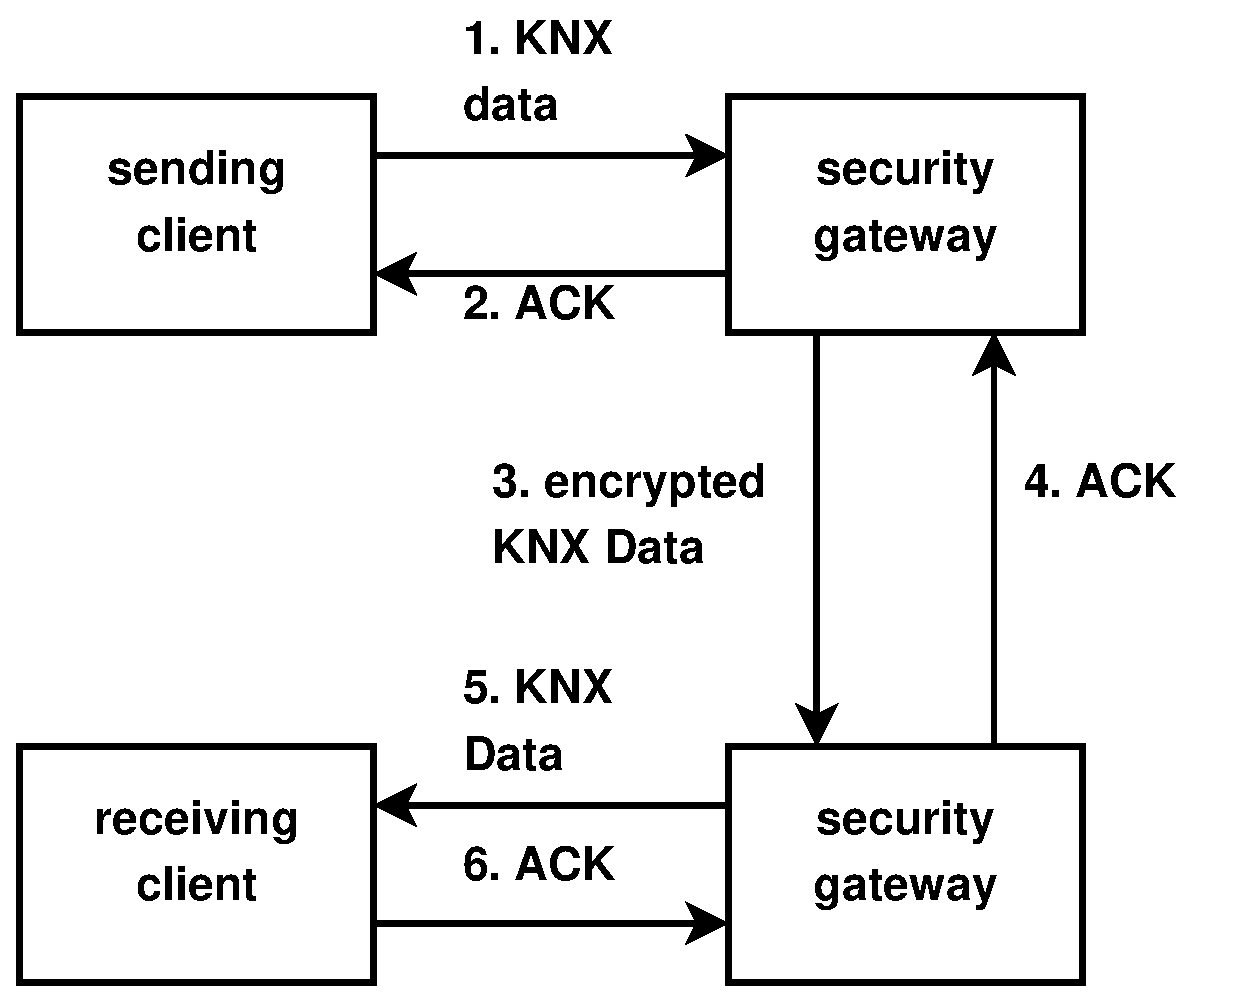
\includegraphics[width=0.6\textwidth]{figures/dataAck.eps}
 \caption{Acknowledgement of KNX data}
 \label{fig:dataAck}
\end{figure}

\section{Services}

\begin{figure}
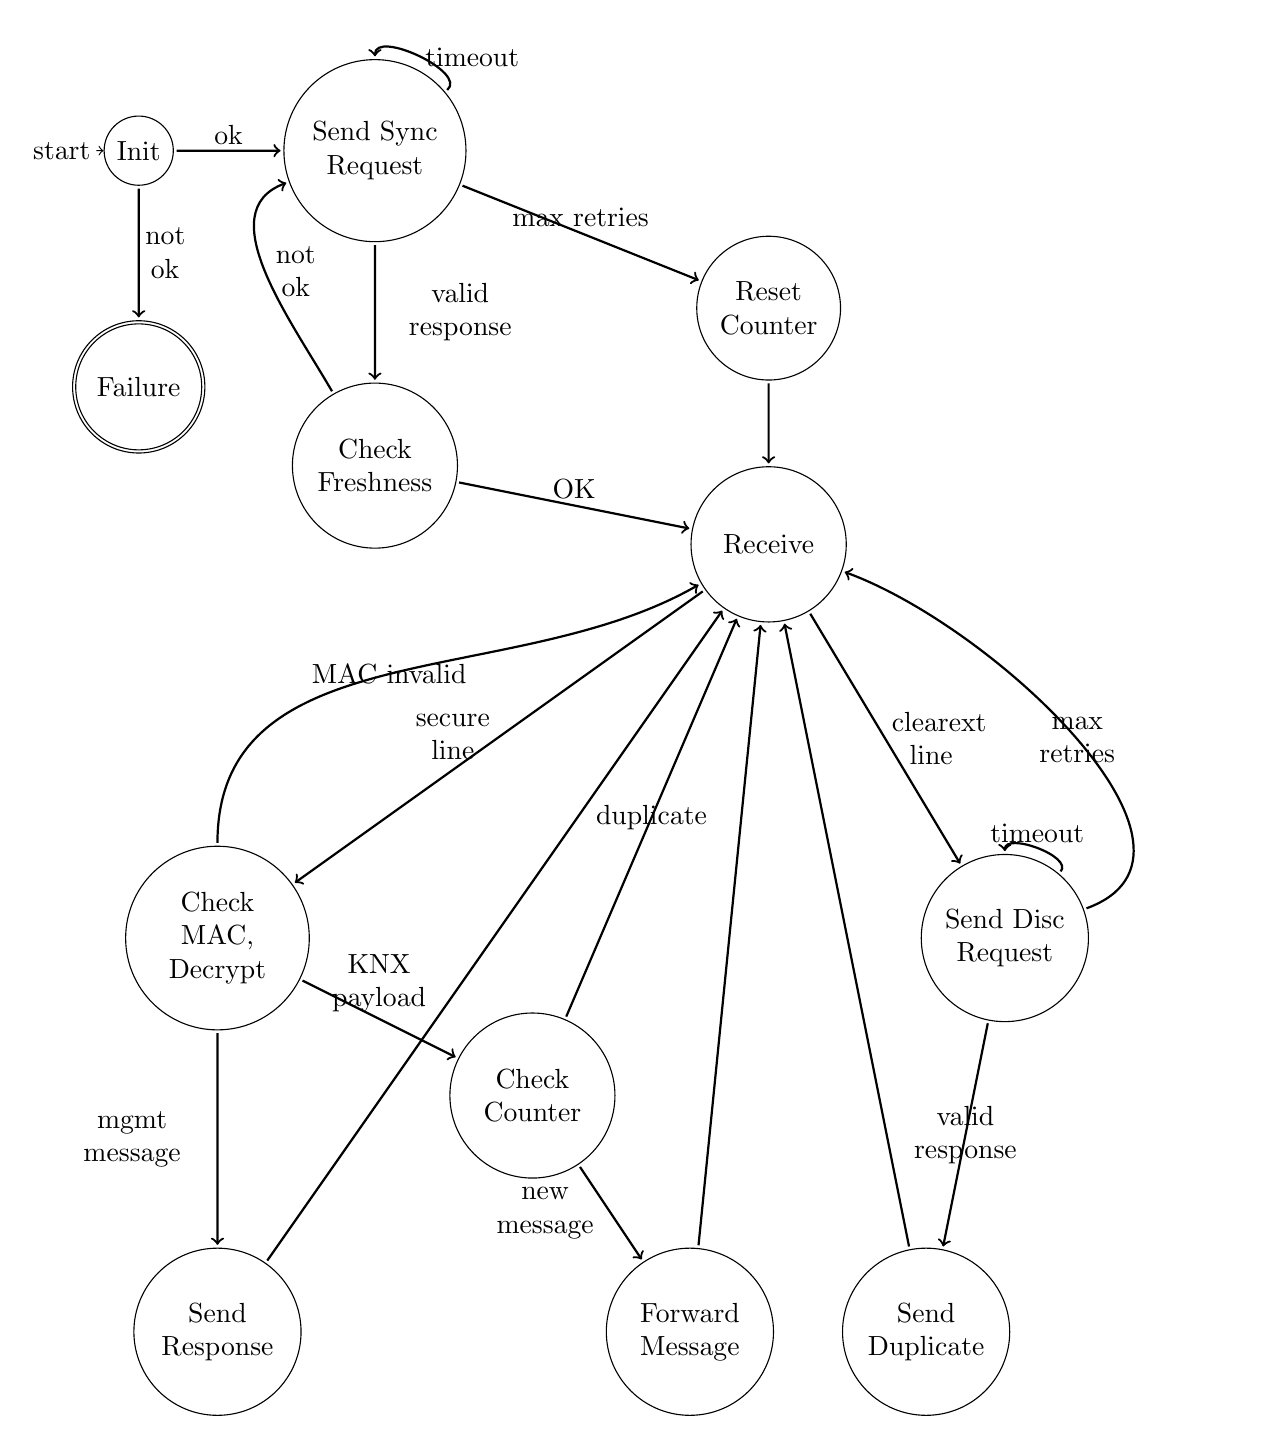
\begin{tikzpicture}[scale=0.2]
\tikzstyle{every node}+=[inner sep=2pt]
\tikzstyle{arrow}=[draw, -latex] 
\tikzset{
    pil/.style={
           ->,
           thick,
           shorten <=1pt,
           shorten >=1pt,}
}

\usetikzlibrary{automata,positioning}
\usetikzlibrary{positioning}

\node[state,initial]												at (45,35)			(init)		{Init}; 
\node[state, text width=2cm,align=center] 	at (60,35)		(sync)	{Send Sync Request};
\node[state, text width=1.5cm,align=center] 	at (45,20)	(fail)	{Failure}; 
\draw [black]	(45,20) circle (4);
\node[state, text width=1.5cm,align=center] 	at (85,25)		(res)	{Reset Counter};
\node[state, text width=1.8cm,align=center] 	at (60,15)		(chkFresh)	{Check Freshness};
\node[state, text width=1.8cm,align=center] 	at (85,10)		(rcv)	{Receive};
\node[state, text width=1.8cm,align=center] 	at (50,-15)		(chkMAC)	{Check MAC, Decrypt};
\node[state, text width=1.8cm,align=center] 	at (100,-15)		(discReq)	{Send Disc Request};
\node[state, text width=1.8cm,align=center] 	at (50,-40)		(sendResp)	{Send Response};
\node[state, text width=1.8cm,align=center] 	at (70,-25)		(chkDup)	{Check Counter};
\node[state, text width=1.8cm,align=center] 	at (80,-40)		(fwd)	{Forward Message};
\node[state, text width=1.8cm,align=center] 	at (95,-40)		(sendDup)	{Send Duplicate};

\path[pil,->] (init)  edge[above] node[text width=1cm,align=center] {ok} (sync); 
\path[pil,->] (init)  edge[right] node[text width=0.5cm,align=center] {not ok} (fail); 
\path[pil,->] (sync)  edge[right,out=40,in=90] node[text width=1cm,align=center] {timeout} (sync); 
\path[pil,->] (sync)  edge[above] node[text width=2cm,align=center] {max retries} (res); 
\path[pil,->] (sync)  edge[right] node[text width=2cm,align=center] {valid response} (chkFresh); 
\path[pil,->] (chkFresh)  edge[right,out=120, in=200] node[text width=0.6cm,align=center] {not ok} (sync); 
\path[pil,->] (res)  edge[above] node[text width=2cm,align=center] {} (rcv); 
\path[pil,->] (chkFresh)  edge[above] node[text width=2cm,align=center] {OK} (rcv); 
\path[pil,->] (rcv)  edge[left] node[text width=1cm,align=center] {secure line} (chkMAC); 
\path[pil,->] (chkMAC)  edge[out=90,in=210] node[text width=2cm,align=center] {MAC invalid} (rcv); 
\path[pil,->] (rcv)  edge[right] node[text width=1cm,align=center] {clearext line} (discReq); 
\path[pil,->] (discReq)  edge[above,out=50,in=90] node[text width=1.2cm,align=center] {timeout} (discReq);
\path[pil,->] (discReq)  edge[] node[text width=2cm,align=center] {valid response} (sendDup); 
\path[pil,->] (discReq)  edge[out=20,in=-20] node[text width=1.5cm,align=center] {max retries} (rcv); 
\path[pil,->] (chkMAC)  edge[left] node[text width=2cm,align=center] {mgmt message} (sendResp); 
\path[pil,->] (sendResp)  edge[left] node[text width=2.5cm,align=center] {} (rcv); 
\path[pil,->] (fwd)  edge[left] node[text width=1cm,align=center] {} (rcv); 
\path[pil,->] (chkMAC)  edge[above] node[text width=1.4cm,align=center] {KNX payload} (chkDup); 
\path[pil,->] (chkDup)  edge[] node[text width=1.5cm,align=center] {duplicate} (rcv); 
\path[pil,->] (chkDup)  edge[left] node[text width=1.5cm,align=center] {new message} (fwd); 
\path[pil,->] (sendDup)  edge[] node[text width=2cm,align=left] {} (rcv); 

\end{tikzpicture}
\label{fig:/statemachines/mainStateMachine}
\caption{State machine of the program logic}
\end{figure}

\subsection{Synchronization service}\label{syncService}

As stated, a new gateway, joining the network, must get knowledge of the actual value of $Ctr_{global}$. This is achieved by sending a broadcast message on
every secure line, 
serving as synchronization request. The frame  contains the device's local time in seconds. The header flags in the secure header are set accordingly, identifying
the frame as synchronization request, see Figure \ref{fig:syncReqFormat}.
\begin{figure}
  \centering
    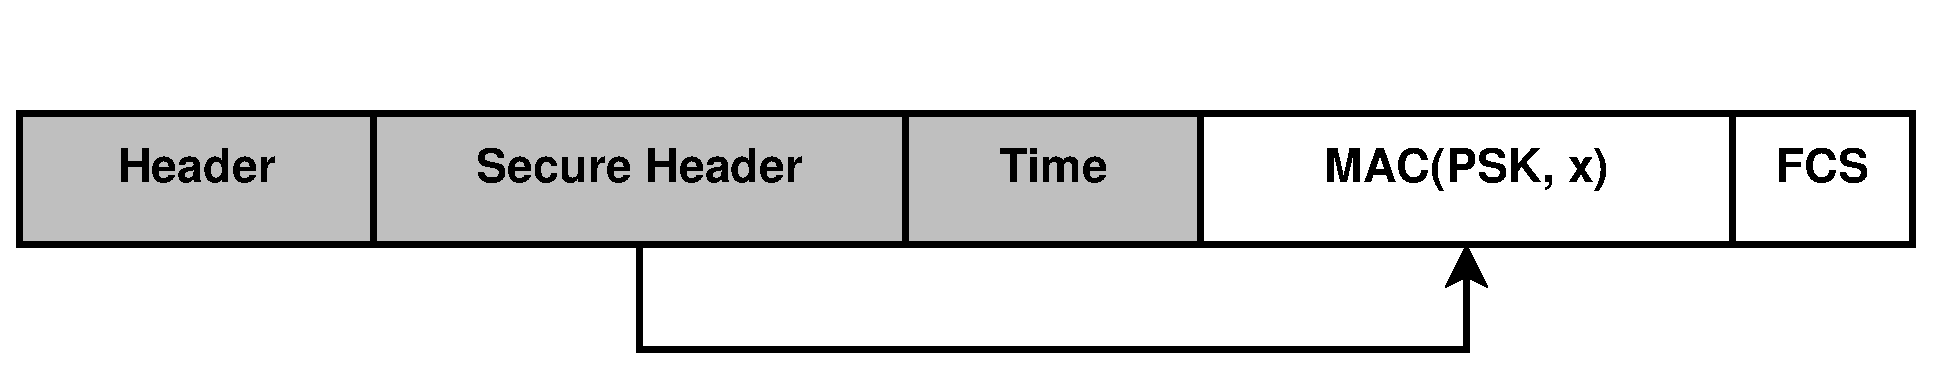
\includegraphics[width=1\textwidth]{figures/formatSyncReq.eps}
 \caption{Synchronization request frame layout}
 \label{fig:syncReqFormat}
\end{figure}
\\
\\
Every device receiving such a request checks the integrity of the message first by recalculating the \gls{mac2}. Afterwards, freshness is checked by comparing
the supplied time with its local time. If the timing information equals the device's own local time, the device sends a unicast synchronization response
frame, containing its local time and the actual counter value. See Figure \ref{fig:syncResFormat} for the layout of such a synchronization response.
The accuracy of the time comparison is deliberately reduced by defining
a window of allowed deviation. This allows a new device to join the network even if its local time and the local time of the answering device are not 
perfectly synchronized.
\begin{figure}
  \centering
    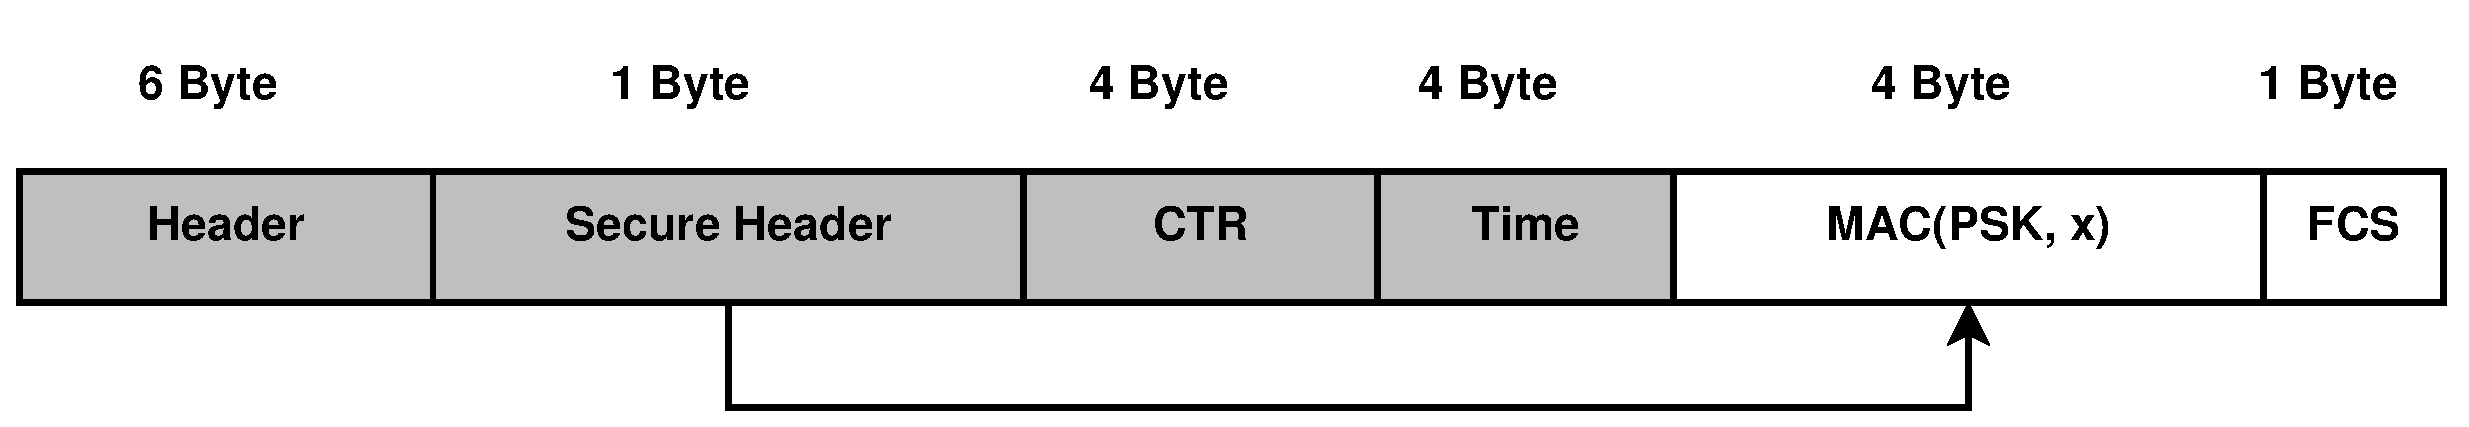
\includegraphics[width=1\textwidth]{figures/formatSyncRes.eps}
 \caption{Synchronization response frame layout}
 \label{fig:syncResFormat}
\end{figure}
If no synchronization response is received within 500ms, up to 2 retries are executed. After that, the device assumes that it is the first device in the
network and resets the global counter $Ctr_{global}$.
\\
\\
The \gls{mac2} is calculated over all frame fields except the trailing frame check fields and parts of the header field. 

\subsection{Discovery service}
Whenever a gateway receives a message on its cleartext line, two distinct discovery broadcast messages are sent, one for each secured line. 
The frame format is shown in Figure \ref{fig:discReqFormat}. DH-A is the newly chosen \gls{ecdh} - parameter of the requesting device.
The \gls{psk} encrypted field contains the group address, CTR contains the incremented global counter $Ctr_{global}$.
\begin{figure}
  \centering
    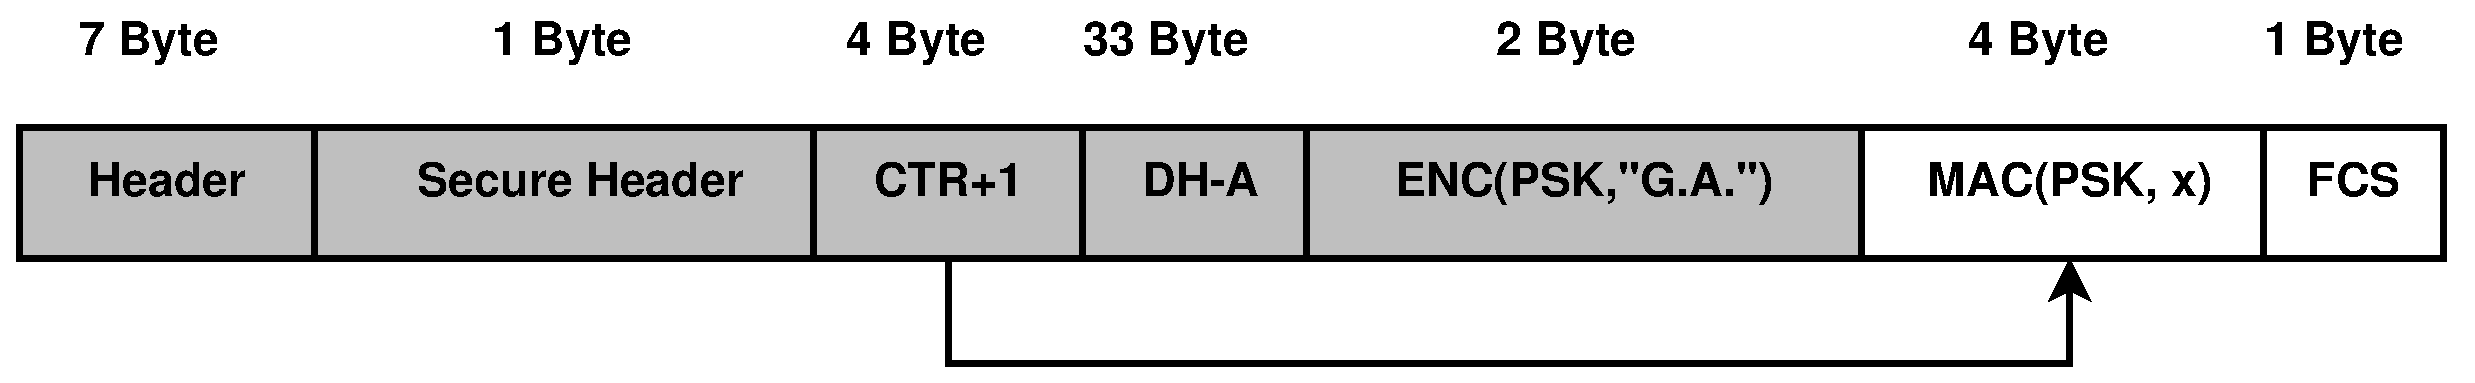
\includegraphics[width=1\textwidth]{figures/formatDiscReq.eps}
 \caption{Discovery request frame layout}
 \label{fig:discReqFormat}
\end{figure}
Every device in the network first checks the authenticity of the received frame by recalculating the \gls{mac2}. If the value differs from the received one, the frame
is discarded. Otherwise, the requested group address is obtained by decrypting the corresponding field, and 
every device recognizing the group address prepares a unicast response frame as shown in Figure \ref{fig:discResFormat}, 
with DH-B as its own newly chosen \gls{ecdh} parameter and the incremented global counter in the CTR field. The requested group address is also
sent, allowing the requester to identify the response message.
\begin{figure}
  \centering
    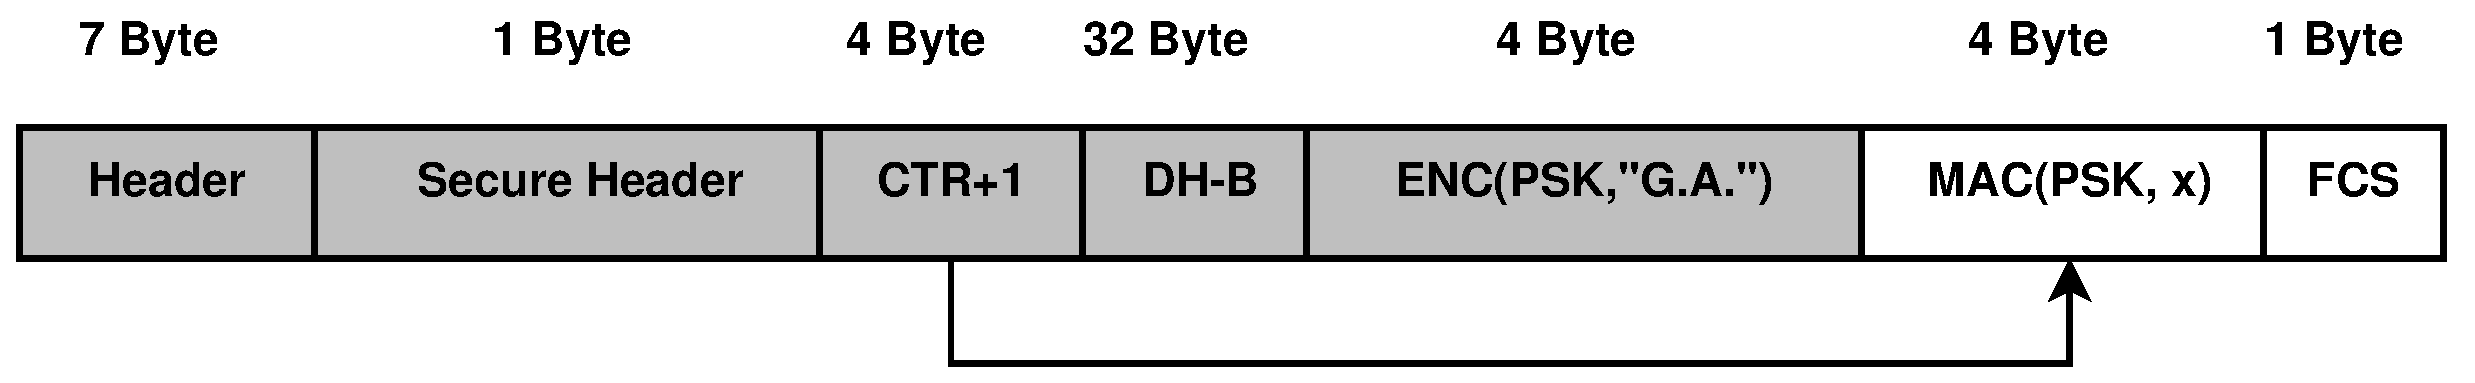
\includegraphics[width=1\textwidth]{figures/formatDiscResp.eps}
 \caption{Discovery response frame layout}
 \label{fig:discResFormat}
\end{figure}
\\
Integrity of the discovery messages is achieved by generating a \gls{mac2} over all frame fields except the frame check field and parts of the header
field. 
\\
The main logic from the discovery request receiver's point of view is shown in the state machine in Figure \ref{fig:discRecv}.

\begin{figure}
\centering
\begin{tikzpicture}[scale=0.2]
\tikzstyle{every node}+=[inner sep=4pt]
\tikzstyle{arrow}=[draw, -latex] 
\tikzset{
    pil/.style={
           ->,
           thick,
           shorten <=1pt,
           shorten >=1pt,}
}

\usetikzlibrary{automata,positioning}
\usetikzlibrary{positioning}

\node[state,initial]												at (15,0)			(rcv)		{Receive}; 
\node[state,text width=1.5cm,align=center]		at (0,-15)		(checkMAC) {Check MAC};
\node[state,text width=1.5cm,align=center]		at (-15,-30)		(discard) {Discard};
\node[state,text width=1.5cm,align=center]		at (15,-30)		(checkCtr) {Check Counter};
\node[state,text width=1.5cm,align=center]		at (0,-45)		(decrypt) {Decrypt};
\node[state,text width=1.5cm,align=center]		at (25,-45)		(sendReply) {Send Reply};

\path[pil,->] (rcv)  edge[] node[text width=1.5cm,align=center] {} (checkMAC); 
\path[pil,->] (discard)  edge[out=90,in=200] node[text width=1.5cm,align=center] {} (rcv); 
\path[pil,->] (checkMAC)  edge[] node[text width=1.5cm,align=left] {MAC invalid} (discard); 
\path[pil,->] (checkMAC)  edge[] node[text width=1.5cm,align=left] {MAC valid} (checkCtr); 
\path[pil,->] (checkCtr)  edge[] node[text width=1.5cm,align=center] {$\le Ctr_{global}$} (discard); 

\path[pil,->] (checkCtr)  edge[] node[text width=1.5cm,align=center] {$> Ctr_{global}$} (decrypt); 
\path[pil,->] (decrypt)  edge[] node[text width=1.5cm,align=center] {GA unknown} (discard); 
\path[pil,->] (decrypt)  edge[] node[text width=1.5cm,align=center] {GA known} (sendReply); 
\path[pil,->] (sendReply)  edge[out=90,in=300] node[text width=1cm,align=right] {} (rcv); 

\end{tikzpicture}
\caption{State machine for processing discovery requests}
\label{fig:discRecv}
\end{figure}

\subsection{Data service}
After receiving one or more discovery responses on one or both secure line, the device which wants to send the \gls{knx} payload (called requester) now knows the
\glspl{ia} which are responsible for delivering messages to the wanted \gls{ga}. The requester can also derive pairwise shared secrets with all responsible gateways, based on \gls{ecdh}.
From this shared secret, a key is derived which is used to encrypt the origin \gls{knx} frame and inserted into the frame after the counter value. This counter $CTR-Ind$ is an individual counter, maintained
by the gateway forwarding the \gls{knx} frame received over the cleartext line.
\\
Authenticity is guaranteed by calculating a \gls{mac2} over all frame fields except the frame check field. The key used for the \gls{mac2} is also derived from the shared secret.
\\
\\
Figure \ref{fig:dataFormat} shows the layout of such a data frame.

\begin{figure}
  \centering
    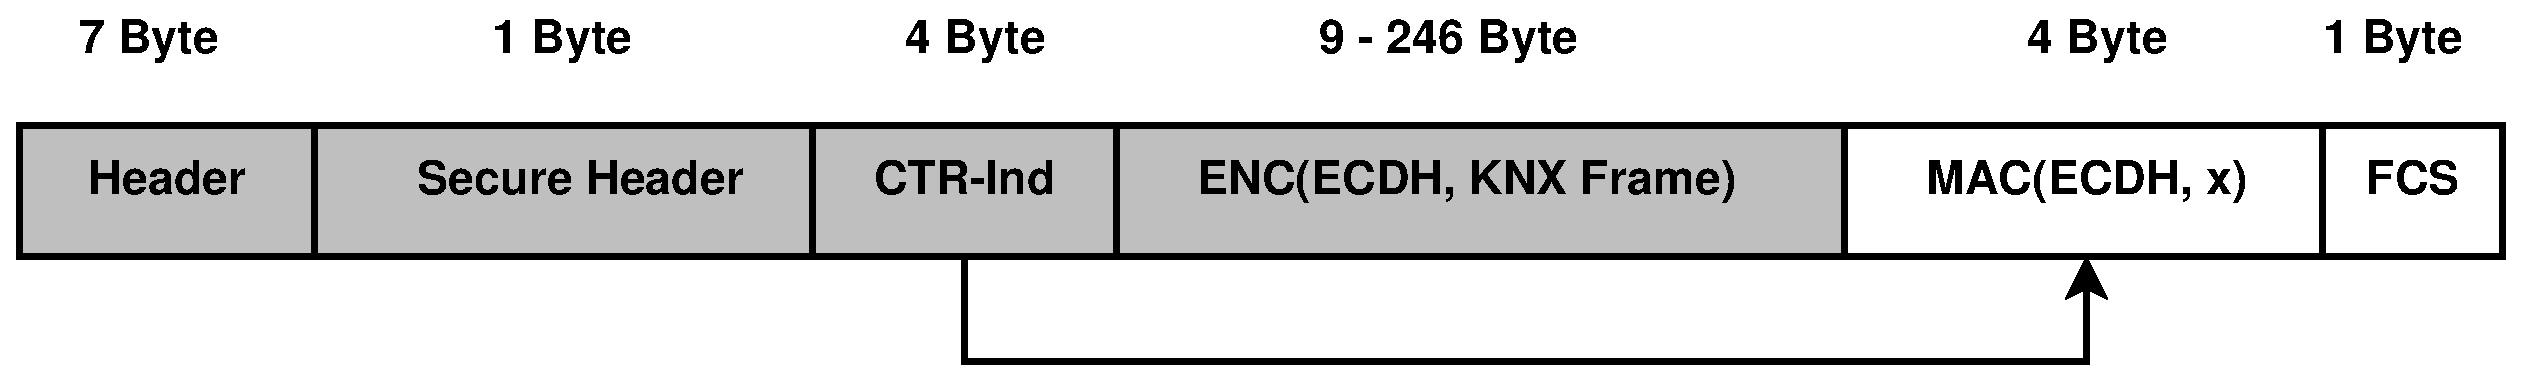
\includegraphics[width=1\textwidth]{figures/formatData.eps}
 \caption{Data  frame layout}
 \label{fig:dataFormat}
\end{figure}

\subsection{Data structures}

The used data structures, referenced above, are introduced in more detail below.

\subsubsection{Secure header}\label{secHdr}
Every frame sent by a security gateway contains a 8 bit header, uniquely determining the type of the frame. Implicitly, this information also determines
the exact type of authentication or authenticated encryption mode used.

\begin{center}
\begin{tabular}{ c | c | c | c}
 \label{table:secHeader}
   bytevalue & frame type & encryption & authentication \\ \hline
   0000 0000 & invalid & x & x \\
   0000 0001 & invalid & x & x \\
   0000 0010 & synchronization request & no & yes \\
   0000 0011 & synchronization response & no & yes \\
   0000 0100 & discovery request & yes & yes \\
   0000 0101 & discovery response & yes & yes \\
   0000 1000 & data service & yes & yes \\
   0000 1001 & reserved & x & x \\
   ...  & ...  & ... & ... \\
   1111 1111 & reserved & x & x \\
\end{tabular}
\end{center}
Values 0x09 - 0xFF are not used - frames containing such values should be discarded.

\subsubsection{Global counter}\label{ctrGlobal}
The global counter $Ctr_{global}$, obtained by the synchronization service and used in the discovery messages,
is a 4 byte integer, allowing $2^{32} \approx 4,3$ billion discovery request or response messages to be sent before overflowing.
This amount is assumed sufficiently high, argued as follows:
each discovery messages consists of a frame containing 53 bytes, sent with 9600 \gls{bps}, resulting in about 44 milliseconds transfer duration. Therefore,
the absolute lower bound of the duration after that $Ctr_{global}$ overflows, assumed the \gls{knx} network is occupied by discovery messages only,
is about two years, a very conservative estimate.

\subsubsection{Individual counter}\label{ctrInd}

Every individual counter is a 4 byte integer, responsible for duplicate detection. Two distinct types of individual counters are used: $Ctr_{out}$, referenced
by an \gls{ia}, and $Ctr_{in}$, also referenced by an \gls{ia}.
Figure \ref{fig:dupSM} shows the state machine describing every security gateway's behavior from a high-level perspective.
\\
Whenever a new \gls{knx} frame is received on the cleartext line and the gateway knows which gateway(s) are responsible for the
contained \gls{ga}, the sending gateway determines the outgoing counter value $Ctr_{out}[\gls{ia}]$. If an outgoing counter value for
this \gls{ia} exists, this means that the device already sent at least one data frame to a \gls{ga}, otherwise this is the first frame. For the first case,
the counter value $Ctr_{out}[\gls{ia}]$ is incremented and saved, otherwise it is set to 1. Afterwards, it is used as value for $Ctr_{ind}$.
After that, the cleartext frame is encrypted and inserted into a new unicast data frame, one for each secure line.
\\
\\
Upon reception (the green transition in Figure \ref{fig:dupSM}), at first the validity of the \gls{mac2} is checked - if valid, the receiver checks its incoming
individual counter value, referenced by the \gls{ia} of the inner frame. If the received counter value $Ctr_{ind}$ is greater than $Ctr_{in}[\gls{ia}]$,
 $Ctr_{ind}$ is saved as $(Ctr_{in}[\gls{ia}]$ and the contained frame (i.e., the \gls{knx} data frame) is forwarded. The second frame, which will be handled 
afterwards will bear the counter value $Ctr_{ind} = Ctr_{in}[\gls{ia}]$ and will be discarded, thus eliminating the duplicate.

\begin{figure}
 \centering
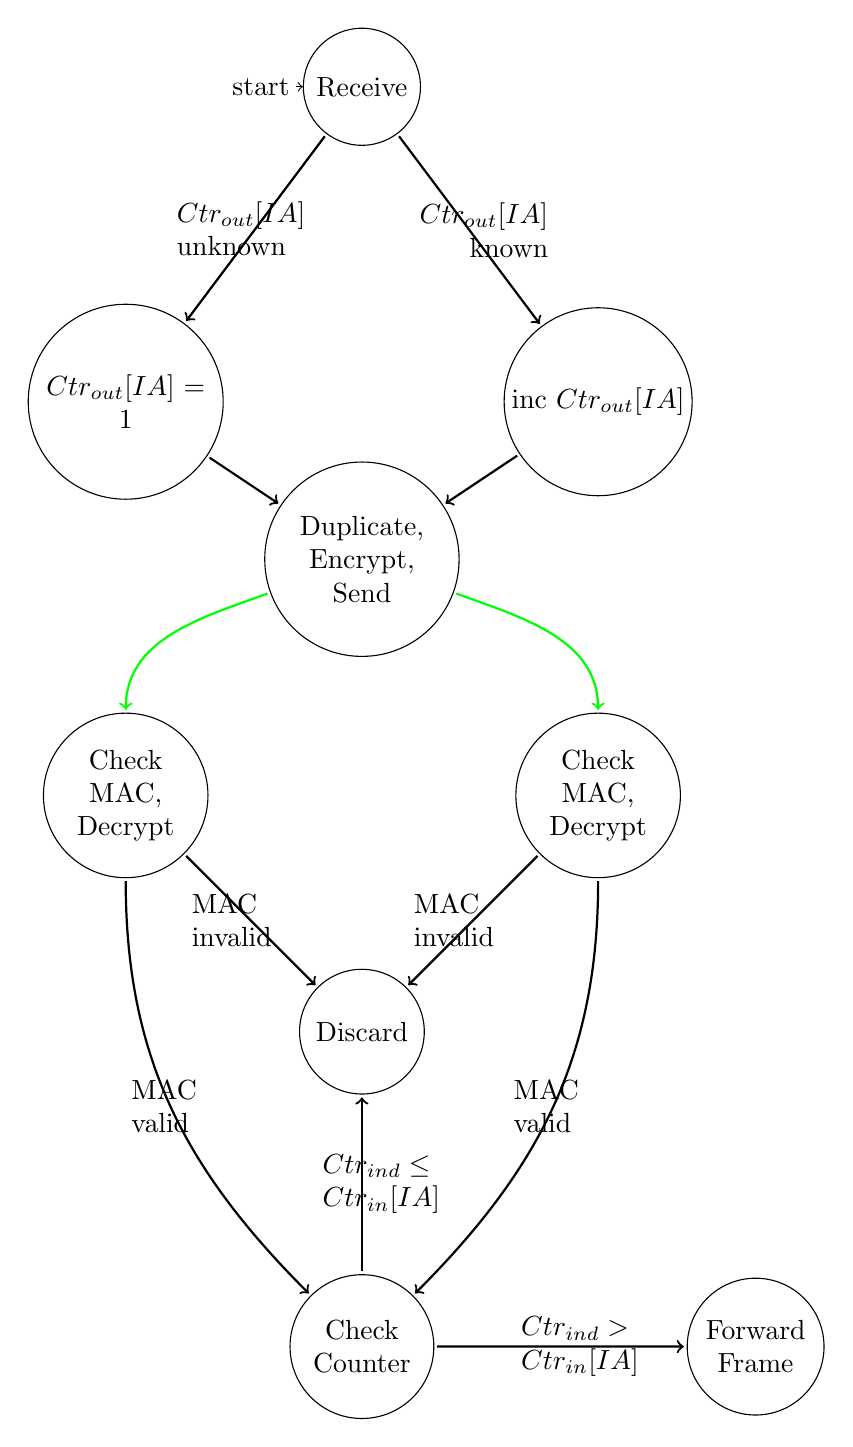
\begin{tikzpicture}[scale=0.2]
\tikzstyle{every node}+=[inner sep=2pt]
\tikzstyle{arrow}=[draw, -latex] 
\tikzset{
    pil/.style={
           ->,
           thick,
           shorten <=1pt,
           shorten >=1pt,}
}

\usetikzlibrary{automata,positioning}
\usetikzlibrary{positioning}

\node[state,initial,text width=1.3cm,align=center]				at (0,-10)		(rcv)		{Receive}; 
%\node[state,text width=2cm,align=center]					at (0,-15)			(chkCtr)	{Check Counter}; 
\node[state,text width=2.2cm,align=center]					at (-15,-30)			(ctrNew)	{$Ctr_{out}[IA] = 1$}; 
\node[state,text width=2.2cm,align=center]					at (15,-30)			(ctrKnown)	{ inc $Ctr_{out}[IA]$}; 
\node[state,text width=2.0cm,align=center]					at (0,-40)			(dup)		{Duplicate, Encrypt, Send}; 
\node[state,text width=1.5cm,align=center]					at (-15,-55)			(rcv1)		{Check MAC, Decrypt}; 
\node[state,text width=1.5cm,align=center]					at (15,-55)			(rcv2)		{Check MAC, Decrypt}; 
\node[state,text width=1.4cm,align=center]					at (0,-70)			(discard)	{Discard}; 
\node[state,text width=1.5cm,align=center]					at (0,-90)			(chk)		{Check Counter}; 
\node[state,text width=1.4cm,align=center]					at (25,-90)			(fwd)		{Forward Frame}; 


\path[pil,->] (rcv)  edge[] node[text width=2cm,align=left] {$Ctr_{out}[IA]$ unknown} (ctrNew); 
\path[pil,->] (rcv)  edge[] node[text width=2cm,align=right] {$Ctr_{out}[IA]$ known} (ctrKnown); 
\path[pil,->] (ctrNew)  edge[] node[text width=1cm,align=right] {} (dup); 
\path[pil,->] (ctrKnown)  edge[] node[text width=3cm,align=right] {} (dup); 
\path[pil,->,color=green] (dup)  edge[out=200,in=90] node[text width=1cm,align=right] {} (rcv1); 
\path[pil,->,color=green] (dup)  edge[out=-20,in=90] node[text width=1cm,align=right] {} (rcv2); 
\path[pil,->] (rcv1)  edge[] node[text width=1.5cm] {MAC invalid} (discard); 
\path[pil,->] (rcv2)  edge[]   node[text width=1.5cm] {MAC invalid} (discard); 
\path[pil,->] (rcv1)  edge[out=270,in=135]   node[text width=1cm] {MAC valid} (chk); 
\path[pil,->] (rcv2)  edge[out=270,in=45]   node[text width=1cm] {MAC valid} (chk); 
\path[pil,->] (chk)  edge[]   node[text width=1cm] {$Ctr_{ind} \le Ctr_{in}[IA]$} (discard); 
\path[pil,->] (chk)  edge[]   node[text width=1cm] {$Ctr_{ind} > Ctr_{in}[IA]$} (fwd); 
% in / out dimension problem...
%\path[pil,->] (fwd)  edge[]   node[] {} (rcv); 

\end{tikzpicture}
\caption{State machine of the duplicate detection logic}
\label{fig:dupSM}
\end{figure}

